\documentclass[12]{article}

\usepackage[margin=1in]{geometry}
\usepackage{setspace}
\usepackage{graphicx}



\begin{document}
\noindent
\onehalfspacing
Jim Vargas \\
CS 162 Programming Assignment 3 \\
\today \\

\begin{center}
Algorithm
\end{center}

	This program will function as a sort of 'proof of concept' database via command line prompts and saving data to text documents. Prompts printed (or outputted) to the command line and commands written (or inputted) to the command line will be the basis for a simple 'general user interface.' The specific theme of this primitive database will involve pets; a user, wishing to store and retrieve information about various animals will be able to use this program to do so.
	
	Let the principle function by which the lesser functions will be linked be designated as 'main' hereon, who's purpose will be to act as the back-end manager. Functions and other important procedures shall be linked to the user via main. Main shall store no permanent data, data shall be filtered into and then out of main.
		
	Let the process by which the user interacts with main be designated as 'GUI' hereon, short for general user interface. GUI will consist of the various prompts which will be printed to the terminal for the user, and will have methods to read in any input should this be appropriate. GUI will be necessity store built in prompts.
	
	Let the database itself be designated as 'ML,' short for master list. ML shall be an external text file stored within accessible range of the program's calling privileges. All data concerning the animals shall be stored, written and retrievable here.
	
\begin{center}
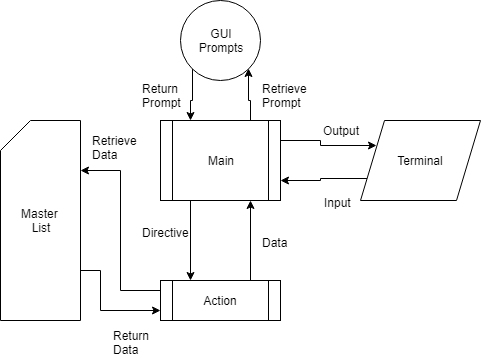
\includegraphics[scale=.8]{data_chart.png}\\
Figure 1: Data Flow Chart
\end{center}

	Figure 1 above describes the look of the program at a high level.

\end{document}